\chapter{Introduction et contexte}


\section{Présentation de l'entreprise}

Il y a 35 ans, Brice Pryszo a fondé MaxSea International en créant le premier logiciel de navigation embarqué
permettant de stocker des cartes marines sur un ordinateur. Depuis, l'entreprise n'a cessé de proposer
des solutions toujours plus innovantes pour les professionnels de la mer, dans plus de 25 pays.
Ses clients comptent des plaisanciers que des pêcheurs ou encore la marine marchande. \\
Elle propose notamment les solutions de navigation TimeZero Navigator (destiné aux plaisanciers)
et TimeZero Professional (destiné aux professionnels de la mer), appuyées par TimeZero Maps,
une cartographie marine de haute qualité.
Ces cartes sont également accessibles sur l'application iOS TimeZero iBoat.
Tous ces produits profitent de leur service météo, qui donne accés à des prévisions
météorologiques et océanographiques très complètes, fournies par les modèles météo les plus fiables.\\

Ces technologies s'appuient sur des appareils d'acquisition haut de gamme, plus particulièrement
ceux fabriqués par Furuno, partenaire principal de la société depuis 2007. Cette collaboration
bénéficie en particulier à TimeZero Coastal Monitoring, qui permet de surveiller les zones côtières. \\

C'est pour ce dernier produit que nous avons effectué notre stage de fin d'études, au sein de l'équipe
de recherche et développement. Plus précisemment, nous avons implémenté un modèle
de détection de navires en temps réel, qui permettra de compléter les informations acquise par le radar
et l'AIS, dont on peut voir un exemple sur la figure ci-après \ref{fig:radar}.

\begin{figure}[H]
    \centering
    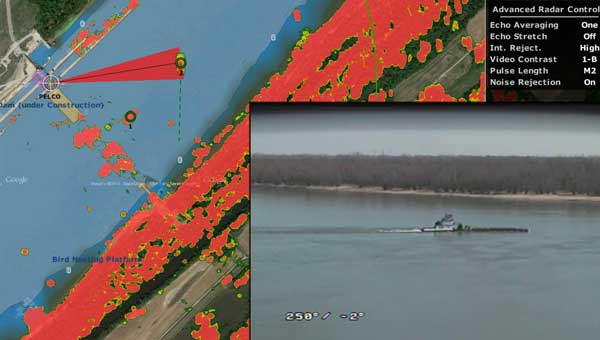
\includegraphics[width=0.8\textwidth]{./img/ports-harbors-cameras1.jpg}
    \caption{Exemple de vue radar, AIS et camera dans TimeZero Coastal Monitoring}
    \label{fig:radar}
\end{figure}

L'équipe que nous avons rejoint était composée de 2 personnes : Ronan Golhen, mon tuteur de stage et
directeur technique, et Victor Opter, développeur logiciel. L'entreprise ne comptant parmi
ses effectifs aucun développeur en apprentissage automatique, nous avons travaillé en autonomie sur le projet,
tout en profitant de la grande expertise métier de mon tuteur, qui connaît non seulement
la partie logiciel, mais qui a de surcroit une grande expérience en navigation.

\section{Début du projet}

Ce projet a commencé en 2023, avec un premier stagiaire qui a travaillé sur la détection de navires. \\

Ses travaux comptent tout d'abord le choix d'un modèle de machine learning nommé YOLOX
(\textit{voir }\ref{yolox}).
Ce choix a été guidé par la recherche de performances, aussi bien du côté de la précision
que de celui de la rapidité, et par des contraintes légales. Ce modèle étant sous
licence Apache 2.0, il est possible de l'utiliser de façon commerciale.\\

Après avoir choisi ce modèle, il a été décidé qu'une phase d'entraînement était nécessaire.
Il a donc récolté des datasets, et réuni environ 8000 images de navires.
Trois entraînements on été réalisés en utilisant des machines distantes via Google Collab. \\

Les résultats du projet comportaient néanmoins quelques limites. Entre autres, les scripts
contenaient un grand nombre de chemins d'accès non relatifs, ce qui rendait
l'exécution difficle. De plus, la documentation très succinte ne permettait pas
de connaître les paramètres exacts utilisés pour l'entraînement. Enfin, l'achat de matériel
spécialisé a rendu obsolète le code relatif à l'utilisation du cloud.\\

Après avoir pris connaissance de ces travaux, nous avons donc entrepris de développer 
un nouvel outil, en utilisant les même librairies que l'année précédente, 
et en écrivant des scripts plus modulaires et en documentant précisément
les étapes de l'entraînement et le code. Ceci a nécessité la maîtrise de l'OS
et du déploiement. 